\documentclass[]{article}
\usepackage{lmodern}
\usepackage{amssymb,amsmath}
\usepackage{ifxetex,ifluatex}
\usepackage{fixltx2e} % provides \textsubscript
\ifnum 0\ifxetex 1\fi\ifluatex 1\fi=0 % if pdftex
  \usepackage[T1]{fontenc}
  \usepackage[utf8]{inputenc}
\else % if luatex or xelatex
  \ifxetex
    \usepackage{mathspec}
  \else
    \usepackage{fontspec}
  \fi
  \defaultfontfeatures{Ligatures=TeX,Scale=MatchLowercase}
\fi
% use upquote if available, for straight quotes in verbatim environments
\IfFileExists{upquote.sty}{\usepackage{upquote}}{}
% use microtype if available
\IfFileExists{microtype.sty}{%
\usepackage{microtype}
\UseMicrotypeSet[protrusion]{basicmath} % disable protrusion for tt fonts
}{}
\usepackage[margin=1in]{geometry}
\usepackage{hyperref}
\hypersetup{unicode=true,
            pdftitle={R Markdown Primer},
            pdfauthor={Erico Cardelli Author},
            pdfborder={0 0 0},
            breaklinks=true}
\urlstyle{same}  % don't use monospace font for urls
\usepackage{color}
\usepackage{fancyvrb}
\newcommand{\VerbBar}{|}
\newcommand{\VERB}{\Verb[commandchars=\\\{\}]}
\DefineVerbatimEnvironment{Highlighting}{Verbatim}{commandchars=\\\{\}}
% Add ',fontsize=\small' for more characters per line
\usepackage{framed}
\definecolor{shadecolor}{RGB}{248,248,248}
\newenvironment{Shaded}{\begin{snugshade}}{\end{snugshade}}
\newcommand{\AlertTok}[1]{\textcolor[rgb]{0.94,0.16,0.16}{#1}}
\newcommand{\AnnotationTok}[1]{\textcolor[rgb]{0.56,0.35,0.01}{\textbf{\textit{#1}}}}
\newcommand{\AttributeTok}[1]{\textcolor[rgb]{0.77,0.63,0.00}{#1}}
\newcommand{\BaseNTok}[1]{\textcolor[rgb]{0.00,0.00,0.81}{#1}}
\newcommand{\BuiltInTok}[1]{#1}
\newcommand{\CharTok}[1]{\textcolor[rgb]{0.31,0.60,0.02}{#1}}
\newcommand{\CommentTok}[1]{\textcolor[rgb]{0.56,0.35,0.01}{\textit{#1}}}
\newcommand{\CommentVarTok}[1]{\textcolor[rgb]{0.56,0.35,0.01}{\textbf{\textit{#1}}}}
\newcommand{\ConstantTok}[1]{\textcolor[rgb]{0.00,0.00,0.00}{#1}}
\newcommand{\ControlFlowTok}[1]{\textcolor[rgb]{0.13,0.29,0.53}{\textbf{#1}}}
\newcommand{\DataTypeTok}[1]{\textcolor[rgb]{0.13,0.29,0.53}{#1}}
\newcommand{\DecValTok}[1]{\textcolor[rgb]{0.00,0.00,0.81}{#1}}
\newcommand{\DocumentationTok}[1]{\textcolor[rgb]{0.56,0.35,0.01}{\textbf{\textit{#1}}}}
\newcommand{\ErrorTok}[1]{\textcolor[rgb]{0.64,0.00,0.00}{\textbf{#1}}}
\newcommand{\ExtensionTok}[1]{#1}
\newcommand{\FloatTok}[1]{\textcolor[rgb]{0.00,0.00,0.81}{#1}}
\newcommand{\FunctionTok}[1]{\textcolor[rgb]{0.00,0.00,0.00}{#1}}
\newcommand{\ImportTok}[1]{#1}
\newcommand{\InformationTok}[1]{\textcolor[rgb]{0.56,0.35,0.01}{\textbf{\textit{#1}}}}
\newcommand{\KeywordTok}[1]{\textcolor[rgb]{0.13,0.29,0.53}{\textbf{#1}}}
\newcommand{\NormalTok}[1]{#1}
\newcommand{\OperatorTok}[1]{\textcolor[rgb]{0.81,0.36,0.00}{\textbf{#1}}}
\newcommand{\OtherTok}[1]{\textcolor[rgb]{0.56,0.35,0.01}{#1}}
\newcommand{\PreprocessorTok}[1]{\textcolor[rgb]{0.56,0.35,0.01}{\textit{#1}}}
\newcommand{\RegionMarkerTok}[1]{#1}
\newcommand{\SpecialCharTok}[1]{\textcolor[rgb]{0.00,0.00,0.00}{#1}}
\newcommand{\SpecialStringTok}[1]{\textcolor[rgb]{0.31,0.60,0.02}{#1}}
\newcommand{\StringTok}[1]{\textcolor[rgb]{0.31,0.60,0.02}{#1}}
\newcommand{\VariableTok}[1]{\textcolor[rgb]{0.00,0.00,0.00}{#1}}
\newcommand{\VerbatimStringTok}[1]{\textcolor[rgb]{0.31,0.60,0.02}{#1}}
\newcommand{\WarningTok}[1]{\textcolor[rgb]{0.56,0.35,0.01}{\textbf{\textit{#1}}}}
\usepackage{graphicx,grffile}
\makeatletter
\def\maxwidth{\ifdim\Gin@nat@width>\linewidth\linewidth\else\Gin@nat@width\fi}
\def\maxheight{\ifdim\Gin@nat@height>\textheight\textheight\else\Gin@nat@height\fi}
\makeatother
% Scale images if necessary, so that they will not overflow the page
% margins by default, and it is still possible to overwrite the defaults
% using explicit options in \includegraphics[width, height, ...]{}
\setkeys{Gin}{width=\maxwidth,height=\maxheight,keepaspectratio}
\IfFileExists{parskip.sty}{%
\usepackage{parskip}
}{% else
\setlength{\parindent}{0pt}
\setlength{\parskip}{6pt plus 2pt minus 1pt}
}
\setlength{\emergencystretch}{3em}  % prevent overfull lines
\providecommand{\tightlist}{%
  \setlength{\itemsep}{0pt}\setlength{\parskip}{0pt}}
\setcounter{secnumdepth}{0}
% Redefines (sub)paragraphs to behave more like sections
\ifx\paragraph\undefined\else
\let\oldparagraph\paragraph
\renewcommand{\paragraph}[1]{\oldparagraph{#1}\mbox{}}
\fi
\ifx\subparagraph\undefined\else
\let\oldsubparagraph\subparagraph
\renewcommand{\subparagraph}[1]{\oldsubparagraph{#1}\mbox{}}
\fi

%%% Use protect on footnotes to avoid problems with footnotes in titles
\let\rmarkdownfootnote\footnote%
\def\footnote{\protect\rmarkdownfootnote}

%%% Change title format to be more compact
\usepackage{titling}

% Create subtitle command for use in maketitle
\providecommand{\subtitle}[1]{
  \posttitle{
    \begin{center}\large#1\end{center}
    }
}

\setlength{\droptitle}{-2em}

  \title{R Markdown Primer}
    \pretitle{\vspace{\droptitle}\centering\huge}
  \posttitle{\par}
    \author{Erico Cardelli Author}
    \preauthor{\centering\large\emph}
  \postauthor{\par}
    \date{}
    \predate{}\postdate{}
  

\begin{document}
\maketitle

{
\setcounter{tocdepth}{2}
\tableofcontents
}
\hypertarget{references}{%
\section{References}\label{references}}

\hypertarget{r-markdown-link-to-topic-notebook}{%
\subsection{R markdown link to topic
notebook}\label{r-markdown-link-to-topic-notebook}}

\href{https://onedrive.live.com/edit.aspx/Documents/Combined\%20Notes?cid=7e1da892b45794cd\&id=documents\&wd=target\%28Technical\%2FTraining.one\%7CE6348C5D-083C-4A40-8324-D42F0B525693\%2FR\%20Markdown\%20Primer\%7C6ED37784-C83D-4E14-B84B-54A6BCD399EC\%2F\%29\%20onenote:https://d.docs.live.net/7e1da892b45794cd/Documents/Combined\%20Notes/Technical/Training.one\#R\%20Markdown\%20Primer\&section-id=\%7BE6348C5D-083C-4A40-8324-D42F0B525693\%7D\&page-id=\%7B6ED37784-C83D-4E14-B84B-54A6BCD399EC\%7D\&end}{Class
OneNote}

\hypertarget{be-contextually-aware}{%
\subsubsection{Be Contextually aware}\label{be-contextually-aware}}

After your metadata section do a ``metasetr'' which will feed new
metadata into new global settings

\begin{Shaded}
\begin{Highlighting}[]
\CommentTok{# Now a snippet to set things right}
\CommentTok{# its funny that outside of this block a comment is a giant Title}

\CommentTok{# This and by using autotab, I was able to piece out}
\CommentTok{# knitr::options for chunks then}
\CommentTok{# RMarkdown is rendering}
\CommentTok{# knitr is evaluating}
\CommentTok{# and the $ is for functions in the knitr opts_chunk function SET (whatever,otherstuff,etc)}
\NormalTok{knitr}\OperatorTok{::}\NormalTok{opts_chunk}\OperatorTok{$}\KeywordTok{set}\NormalTok{(}\DataTypeTok{cache=}\OtherTok{TRUE}\NormalTok{, }\DataTypeTok{fig.align =} \StringTok{'center'}\NormalTok{, }\DataTypeTok{echo =} \OtherTok{TRUE}\NormalTok{)}
\end{Highlighting}
\end{Shaded}

\hypertarget{my-first-section}{%
\section{My First Section}\label{my-first-section}}

We start a new section with a single HASHTAG and this is the first
paragraph in that section. Notice how the text wraps around to the next
line in the editor but it still has the same line number and that's
pretty cool. That's because all text on a single line is considered a
paragraph.

Leaving a blank line starts a new paragraph. Remember Markdown is highly
spaced and cased aware. If you don't leave a blank line you are still in
the same paragraph

So it is very important to pay attention to spaces.

F7 for spell check.

\hypertarget{new-section}{%
\section{New Section}\label{new-section}}

You start a new section by leaving a blank line and then starting the
next line with a hash tag. No need to close the previous section, just
start a new one. (Similar to La-Tex)

\hypertarget{subsections}{%
\section{Subsections}\label{subsections}}

Creating a subsection is easy. Two Hash tags

\hypertarget{this-is-a-subsection}{%
\subsection{This is a Subsection}\label{this-is-a-subsection}}

We start a section in a section to start it

You can use add decorator module

\hypertarget{another-subsection}{%
\subsection{Another Subsection}\label{another-subsection}}

Same rules apply no need to close previous subsection just keep a blank
line in between them

the output type is actually an R function you are specifying and is in
the R Markdown Package

\hypertarget{back-to-sections}{%
\section{Back to Sections}\label{back-to-sections}}

\hypertarget{formatting-text}{%
\section{Formatting Text}\label{formatting-text}}

One Underline is for \emph{Emphasized}

\emph{Emphasized Words Go Here}

Strong Text is with two underlines \textbf{Strong}

\textbf{Strong Text Goes Here}

And you can combine them with Three Underlines \textbf{\emph{Bold and
Strong}}

And finally code snippets are the BACKTIC under the Esc

\texttt{This\ is\ computer\ Code}

\hypertarget{lists}{%
\section{Lists}\label{lists}}

\hypertarget{unordered-list}{%
\subsection{Unordered List}\label{unordered-list}}

Fruit

\begin{itemize}
\tightlist
\item
  Apple
\item
  Orange
\item
  Banana
\item
  Mango
\item
  Durian
\item
  Watermellon
\item
  Dragonfruit
\end{itemize}

\hypertarget{ordered-list}{%
\subsection{Ordered List}\label{ordered-list}}

To createa an ordered list use 1. at the beginning of your list items
Hit Dice and a sublist with a. to make the sublist

\hypertarget{sublists}{%
\subsubsection{Sublists}\label{sublists}}

I added subs in there too

\begin{enumerate}
\def\labelenumi{\arabic{enumi}.}
\tightlist
\item
  Bug

  \begin{enumerate}
  \def\labelenumii{\alph{enumii}.}
  \tightlist
  \item
    gnat
  \item
    fly
  \item
    spider
  \item
    wasp
  \end{enumerate}
\item
  Fool

  \begin{enumerate}
  \def\labelenumii{\roman{enumii}.}
  \tightlist
  \item
    dope
  \item
    idiot
  \end{enumerate}
\item
  Knight
\item
  Troll
\item
  Dragon
\end{enumerate}

\hypertarget{links}{%
\section{Links}\label{links}}

You put the text you want displayed in square brackets and then the url
into parenthesis

\texttt{{[}Google{]}(https://www.google.com)} =
\href{https://www.google.com}{Google}

\href{https://onedrive.live.com/edit.aspx/Documents/Combined\%20Notes?cid=7e1da892b45794cd\&id=documents\&wd=target\%28Technical\%2FTraining.one\%7CE6348C5D-083C-4A40-8324-D42F0B525693\%2FR\%20Markdown\%20Primer\%7C6ED37784-C83D-4E14-B84B-54A6BCD399EC\%2F\%29\%20onenote:https://d.docs.live.net/7e1da892b45794cd/Documents/Combined\%20Notes/Technical/Training.one\#R\%20Markdown\%20Primer\&section-id=\%7BE6348C5D-083C-4A40-8324-D42F0B525693\%7D\&page-id=\%7B6ED37784-C83D-4E14-B84B-54A6BCD399EC\%7D\&end}{Class
OneNote}

\hypertarget{r-time}{%
\section{R Time!!!!}\label{r-time}}

\emph{Alt+Ctrl+I for new code chunk}

\begin{Shaded}
\begin{Highlighting}[]
\DecValTok{1}\OperatorTok{+}\DecValTok{1}
\end{Highlighting}
\end{Shaded}

\begin{verbatim}
## [1] 2
\end{verbatim}

R Markdown showed you the code, executed cleanly, and displays results

\begin{Shaded}
\begin{Highlighting}[]
\CommentTok{# this is a comment inside of R code}
\CommentTok{# here I will set a variable that is only inside this code bubbles}
\NormalTok{x<-}\DecValTok{3}
\NormalTok{x}
\end{Highlighting}
\end{Shaded}

\begin{verbatim}
## [1] 3
\end{verbatim}

\hypertarget{text-in-between-code-such-heresy}{%
\section{Text in between code? Such
Heresy}\label{text-in-between-code-such-heresy}}

\begin{Shaded}
\begin{Highlighting}[]
\NormalTok{x}\OperatorTok{*}\DecValTok{2}
\end{Highlighting}
\end{Shaded}

\begin{verbatim}
## [1] 6
\end{verbatim}

Chunks are cumulative and serial but not in any way related to the
console or any other \texttt{ENVIRONMENT}

\hypertarget{naming-chunks}{%
\section{Naming Chunks?}\label{naming-chunks}}

So in the code chunk right after the r that defines it as
\texttt{R\ Code} put a space and then a name followed by the other
curlybrace See the Example here

\begin{Shaded}
\begin{Highlighting}[]
\NormalTok{x}\OperatorTok{*}\DecValTok{7}\OperatorTok{+}\DecValTok{3}
\end{Highlighting}
\end{Shaded}

\begin{verbatim}
## [1] 24
\end{verbatim}

Lets show the results of a code chunk without showing the code

\begin{verbatim}
## [1] 19
\end{verbatim}

by doing echo=false the code is safely hidden but results flow

look to the left and you can see carrots that let you fold the stuffs

\hypertarget{better-examples}{%
\subsection{Better Examples}\label{better-examples}}

Alt+Shift+K will show you keyboard Shortcuts

\hypertarget{plots}{%
\section{Plots}\label{plots}}

Plots all make sense of data but first we have to prepare for the plots
And loading more prerequisites

\begin{Shaded}
\begin{Highlighting}[]
\KeywordTok{library}\NormalTok{(ggplot2)}
\end{Highlighting}
\end{Shaded}

Put the library code alone to enable smart reuse

\begin{Shaded}
\begin{Highlighting}[]
\KeywordTok{ggplot}\NormalTok{(diamonds, }\KeywordTok{aes}\NormalTok{(}\DataTypeTok{x=}\NormalTok{carat, }\DataTypeTok{y=}\NormalTok{price, }\DataTypeTok{color=}\NormalTok{cut)) }\OperatorTok{+}\StringTok{ }\KeywordTok{geom_point}\NormalTok{()}
\end{Highlighting}
\end{Shaded}

\begin{center}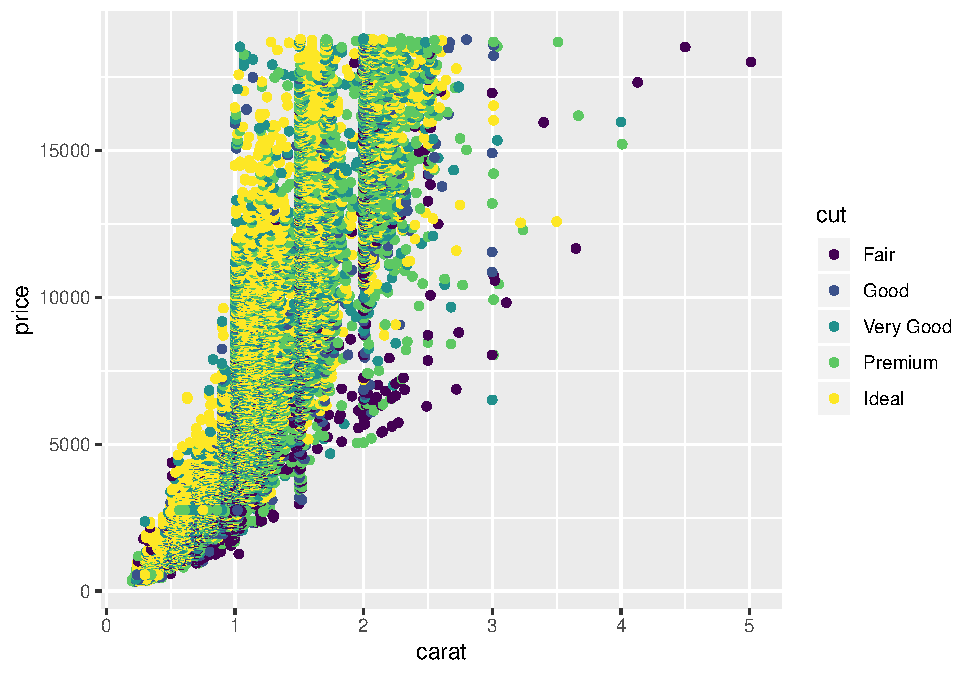
\includegraphics{rmarkdown_primer_ec_files/figure-latex/unnamed-chunk-4-1} \end{center}

\emph{What is amaziing about this is that the picture is embeded as a
graphic but its encoded so anyone can see it and all the images are
embedded}

\hypertarget{including-javascript}{%
\section{Including Javascript}\label{including-javascript}}

The web page actually embeds everything for your use

\hypertarget{plot-improvements}{%
\section{Plot Improvements}\label{plot-improvements}}

I want to center the plot\ldots{}

\begin{Shaded}
\begin{Highlighting}[]
\KeywordTok{ggplot}\NormalTok{(diamonds, }\KeywordTok{aes}\NormalTok{(}\DataTypeTok{x=}\NormalTok{carat, }\DataTypeTok{y=}\NormalTok{price, }\DataTypeTok{color=}\NormalTok{cut)) }\OperatorTok{+}\StringTok{ }\KeywordTok{geom_point}\NormalTok{()}
\end{Highlighting}
\end{Shaded}

\begin{center}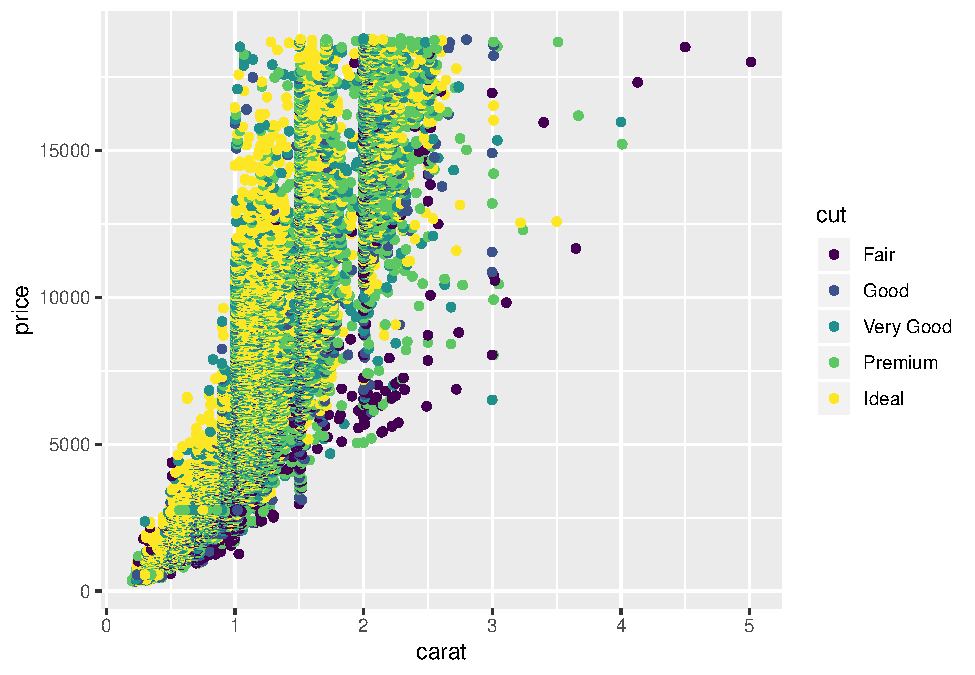
\includegraphics{rmarkdown_primer_ec_files/figure-latex/Align-my-diamonds-plot-1} \end{center}

The alignment directive in that code was easy to figure out with the
comma intellisyntax

\hypertarget{a-caption}{%
\subsection{A Caption}\label{a-caption}}

\begin{Shaded}
\begin{Highlighting}[]
\KeywordTok{ggplot}\NormalTok{(diamonds, }\KeywordTok{aes}\NormalTok{(}\DataTypeTok{x=}\NormalTok{carat, }\DataTypeTok{y=}\NormalTok{price, }\DataTypeTok{color=}\NormalTok{cut)) }\OperatorTok{+}\StringTok{ }\KeywordTok{geom_point}\NormalTok{()}
\end{Highlighting}
\end{Shaded}

\begin{figure}

{\centering 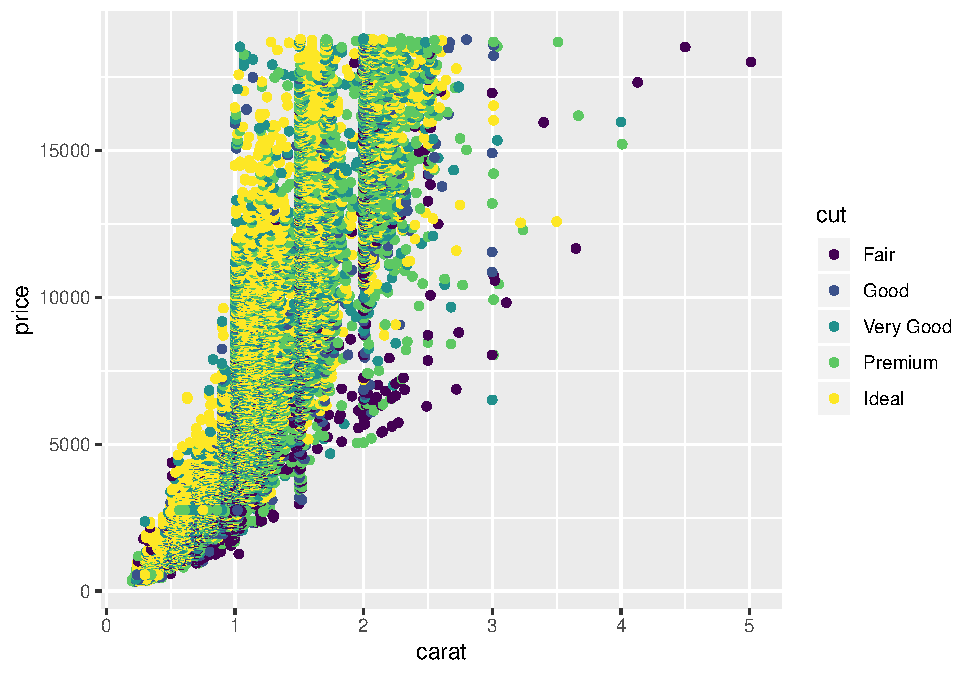
\includegraphics{rmarkdown_primer_ec_files/figure-latex/plot-diamond-with-caption-1} 

}

\caption{A scatterplot of diamond price vs. size, color coded according to diamond cut}\label{fig:plot-diamond-with-caption}
\end{figure}

Lots to unpack in this code\ldots{} but where it sayd cache=TRUE, that
means that if this code snippet hasn't changed use it as is. possibly
saving a lot of time


\end{document}
